\documentclass[runningheads,a4paper]{article}

\usepackage[utf8]{inputenc}

\setcounter{tocdepth}{3}

\usepackage[english]{babel} 
\usepackage{graphicx}
\usepackage{grffile}
\usepackage{float}
\usepackage{multicol}
\usepackage{url}
\usepackage{array}
\usepackage{wrapfig}
 \usepackage{multirow}
\usepackage{tabu}
\usepackage{amssymb}% http://ctan.org/pkg/amssymb
\usepackage{pifont}% http://ctan.org/pkg/pifont
\usepackage[font=small,labelfont=bf]{caption}

\newcommand{\cmark}{\ding{51}}%
\newcommand{\xmark}{\ding{55}}%

\usepackage{titling}
\usepackage[hidelinks]{hyperref}
\setcounter{secnumdepth}{5}
%Margins
\usepackage[
margin=2cm,
includefoot
]{geometry}


\graphicspath{{/}}

%Headers and Footers
\usepackage{fancyhdr}
\pagestyle{fancy}
\fancyhead{}
\fancyfoot{}
\fancyfoot[R]{\thepage}
\renewcommand{\headrulewidth}{0pt}
\renewcommand{\footrulewidth}{0pt}
\setlength\parindent{24pt}
\begin{document}
	
%Title Page
\begin{titlepage}
	\begin{center}
		
\includegraphics[width=10cm]{UP_Logo.PNG}  \\
		[1cm]
		\line(1,0){300} \\
		[0.3cm]
		\textsc{\Large
			Benchmarking Service\\
			Software Requirements Specification\\
			\hfill
			%University of Pretoria
		}\\
		[0.1cm]
		\line(1,0){300} \\
		[0.7cm]
		\textsc{\Large
			ProCoders
		} \\
	\end{center}
	
	\begin{center}
		\begin{centre}
			\textsc{\large\\
				Bongani Tshela - 14134790\\ 
			}
		
				\textsc{\large\\
					Harris Leshaba - 15312144\\ 
				}
			\textsc{\large\\
				Joseph Letsoalo - 15043844\\ 
			}
			
			\textsc{\large\\
				Minal Pramlall - 13288157\\ 
			}
			

            

		\end{centre}
		
		
		
	\end{center}
\end{titlepage}
%\maketitle%%%%%%%%%%%%%%%%%%%%%%%%%%%%%%%%%%%%%%%%%%%%%%%%%%%%%%%%%%%%%%%%%%%%

\begingroup

\tableofcontents
\addcontentsline{toc}{section}{Table Of Contents}
\endgroup
\newpage
\section{Project background.}
Bench marking seem to be a very common and useful application, very few bench-marking tools or services are available. Those that are available requires intricate configuration that may be beyond the reach of the developers, researchers,
teachers and students who would like to use them. The development of a bench-marking service which can be used in a generic way would therefore be welcomed by a large
potential user base.

\section{Project vision.}
The system provides a web interface for users to request and specify the bench-marking services they need. The services will be provided by executing the requested benchmarks on isolated machines where the side-effects that are not a concern of the specified benchmark is minimized. The system measures a variety of performance attributes such as CPU time, elapsed time, memory usage, power consumption, heat generation, etc. Ir accepts source code for a variety modern programming languages.
\section{Project Scope}
The core of the system is a benchmarking tool which. The high level modules and their responsibilities are
shown in Figure 1
\section{User management module}
\subsection{Scope}
The scope of the user management module is shown in Figure 1. The user
management module is responsible for maintaining information about the registered
users of the system, including the authority levels of each user. User can manage their benchmarking records like deleting and storing new records, view them and retrieving old algorithm they have stored.

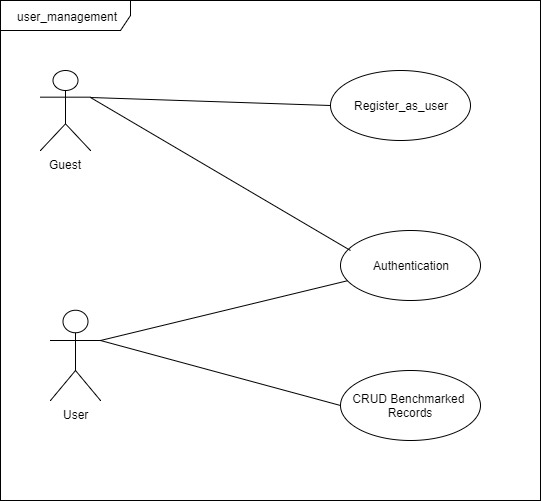
\includegraphics[width=7cm,height=10cm]{userDiagram.jpg}
\newline 
\textit{Figure 1} use case.
\newline
\newline No information is stored for the guest user. When accessing the service, the user
assumes the guest role without being logged in. The guest user may use public
services and my register or log in.
When a user is registered, the fields shown in the domain model are stored for the
user using a unique automatically assigned ID. The user provides all other fields. The
password is stored in encrypted format. The user can access all the services provided by the service
The register as user  use case is initiated by an end-user to create an account.\newline\newline
A user will not be created if the email specified in the request to create a user is already
associated with an existing user. This is done to ensure that if a user is already associated
with the email address, the user is given access to his/her profile instead of creating a new
user.\newline\newline
Note that this use case will use the \textbf{getUser(userEmail)} service provided by the module to
confirm if another user with that same email already exists in the system. A user should
only be created if \textbf{getUser(userEmail)} throws the \textit{noSuchUser} exception.
After the account has been created a notification will be sent to the user. The system have two types of users: Guest user and Registered user.
\subsubsection{\textbf{Domain model}}
The users management domain model is shown in Figure 2
\newline
\newline
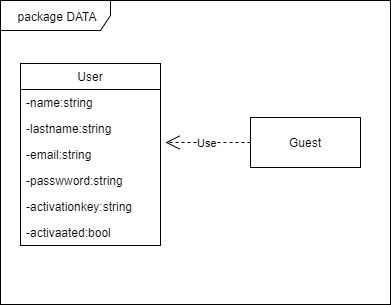
\includegraphics[width=7cm,height=8cm]{userClass.jpg}
\newline 
\textit{Figure 2} class diagram.

\subsubsection{\textbf{Precondition Table}}
CU1 \textbf{getUserEmail(email)}
\newline
\newline
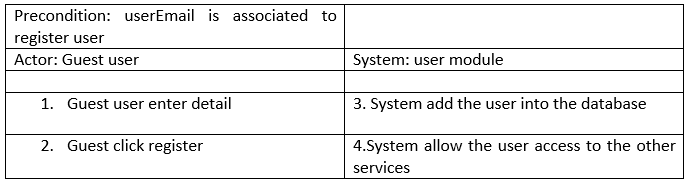
\includegraphics[width=12cm,height=3cm]{preUser.PNG}
\newline 
\textit{Figure 3} class diagram.

\subsection{\textbf{Service contracts}}
The following services should be provided
\newline
\newline
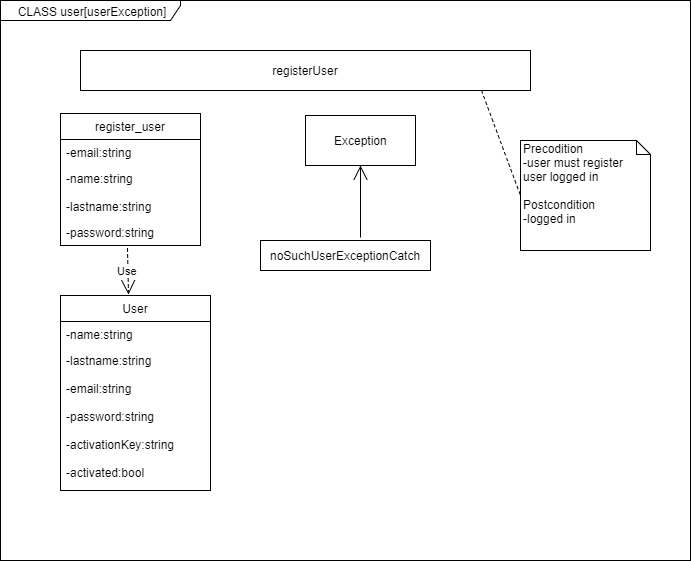
\includegraphics[width=12cm,height=10cm]{userConstract.jpg}
\newline 
\textit{Figure 4} class diagram.

\section{Display module}
\subsection{Scope}
The display module construts graphs, charts and tables to represent the benchmark results, and how different algorithms 
compare against one another in terms of perfolrmance.

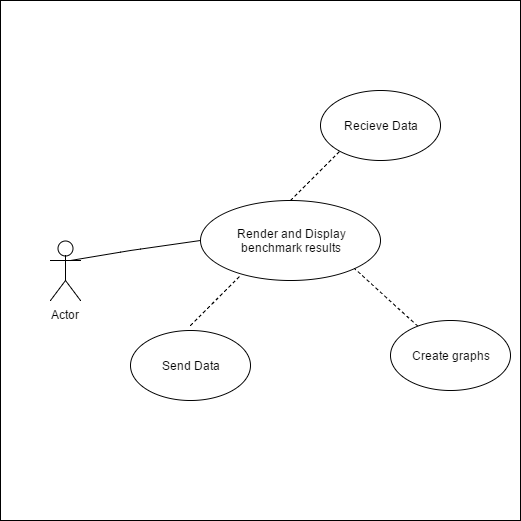
\includegraphics[width=7cm,height=10cm]{DisplayUseCase.png}
\newline 
\textit{Figure 5} use case.
\newline
\newline
The display module concerns itself with rendering and displaying the results of benchmarks.
The display module concerns itself primarily about creating graphs, charts and tables to represent the
benchmarking results in a easily readable manner. 
\newline
\subsubsection{\textbf{Domain model}}
The Display domain model is shown in Figure 6
\newline
\newline
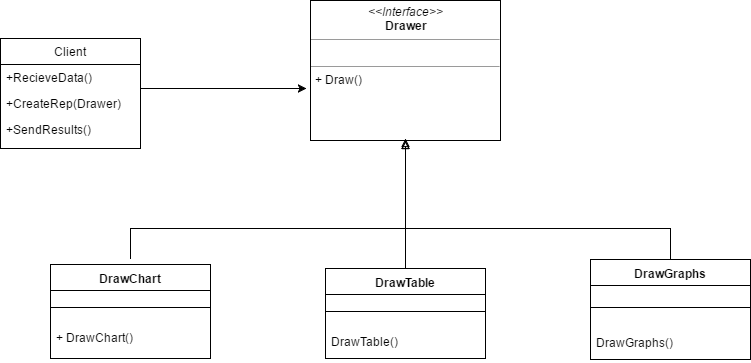
\includegraphics[width=7cm,height=8cm]{DisplayDomainModel.png}
\newline 
\textit{Figure 6} class diagram.
\newline
The domain model indicates how the client will use the Drawer to create the specific representation of the benchmark results.
\newline
\subsection{\textbf{Service contracts}}
The following services should be provided
\newline
\newline
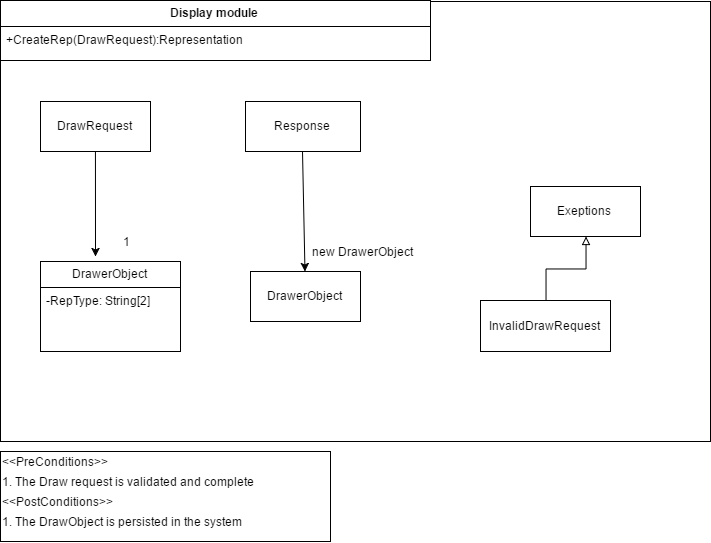
\includegraphics[width=12cm,height=10cm]{DisplayServiceContracts (1).png}
\newline 
\textit{Figure 7} Service Contracts.
\newline
The service contract specified above will be refused under one condition. If the draw request fails the validation protocol, 
then the contract can be refused. Otherwise, the DrawObject will be persisted and stored in the system.
\newline
\subsection{\textbf{Technologies}}
\newline
When it comes to Display technologies, one in particular is of note.
 JFreeChart - A free 100% JAVA chart library that makes it easy for developers to display professional quality charts in their applications.
 JFreeChart's extensive feature set includes:
	\item 1.A consistent and well-documented API, supporting a wide range of chart types;
	\item 2.A flexible design that is easy to extend, and targets both server-side and client-side applications;
	\item 3.Support for many output types, including Swing and JavaFX components, image files (including PNG and JPEG), and vector graphics file formats (including PDF, EPS and SVG);
	\item 4.JFreeChart is open source or, more specifically, free software. It is distributed under the terms of the GNU Lesser General Public Licence (LGPL), which permits use in proprietary applications.
	
\section{Bench-marking and VM initializing Module}
\subsection{Scope}

The module initializes and deploys VMs based on the request(s). On the VMs we will have a Java program that runs other programs, that is compile them, run them with the user specified data sets and then benchmark the program or algorithms. This module will initialize VMs on request and can initialize them concurrently within seconds.\\

\includegraphics[width=15cm , height=12cm]{VMInitialier.jpg}  \\
\subsection{Service Contracts.}
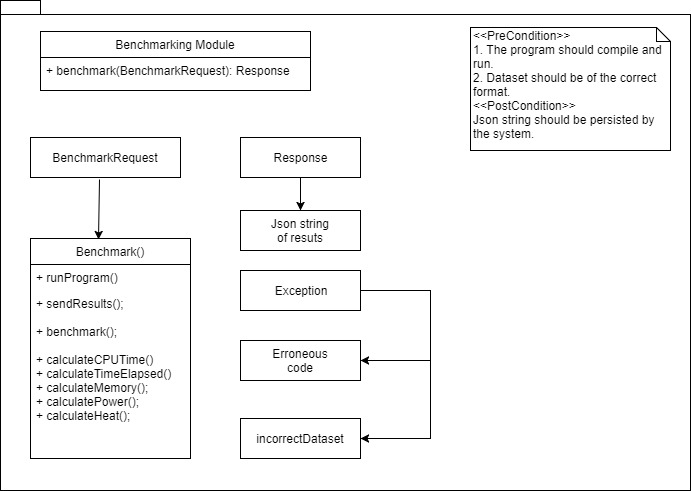
\includegraphics[width=15cm , height=12cm]{SCBenchmark.jpg}  \\
\subsection{Technologies.}
Osv - the open source operating system designed for the cloud. Built from the ground up for effortless deployment and management, with superior performance.\\

Unikernels - specialized, single address space machine images constructed by using library operating systems(Osv in our case).We select, from a modular stack, the minimal set of libraries which correspond to the OS constructs required for our application to run.\\
\end{document}


